%!TEX root = ../deco_star.tex


\section{Analysis of the State of the Art}
\label{sec:analysis}

% In this section, we execute the above established analysis framework in regard to creative control for pattern generation. 

The contribution of this survey is twofold. On the one hand, its analysis the state of the art with regard to control mechanisms, translates this categorization to overall control paradigms and discusses their means for creative control. On the other hand, it selects the work not by its underlying algorithms and creation techniques but by its design goal, namely creative pattern generation. This type of pattern generation includes a variation of representative creation challenges, such as combining ordered fillings and repetitive structures with individual frames or lining and highlighting components that might break with an underlying repetitive structure. The focus on the visual output instead of specific underlying algorithms allows for a novel and unifying discussion of techniques and merges a discussion of work that is traditionally studied separately. Thus this focus furthers a common understanding of creative control mechanisms.

The analysis of the control mechanisms is directly taken from the authors' descriptions. However, the following discussion of the creative means has an interpretative nature to it. Despite our best efforts to give a clear reasoning, we also agree that this is not always unambiguously manageable. Thus, this discussion should be viewed as a step toward an objective discussion about terms such as artist-usable and creatively controllable as well as a more realistic usage of these terms.


\subsection{Commonly Used Controls}
\label{subsec:commonly_used_control_mechanisms}

\minortodo[inline]{Add intro}

\subsubsection{Example-Based Control}
\label{subsubsec:commonly_used_control_mechanisms_example}

On of the most prominently investigated techniques for texturing are example-based approaches. Example-based control mechanisms compute a separate output based on a given example and provide a \textit{goal-oriented control}. The motivation behind using these techniques is mainly to generate a specific and predictable output as efficiently as possible. Example-based and inverse approaches have a long history in the control of procedural representations. They remain a dominant research field and are relevant for any discussion about controlling procedural models. 

In regard to creative control, example-based approaches detach the design task to a data-driven image generation techniques, such as taking a photograph or designing a sample in an application such as Adobe Photoshop or Illustrator.

Relevant factors for differentiating example-based techniques are the size of the design space, hence their expressiveness, performance and initialization requirements. The following investigation is roughly sorted by increasing expressiveness.

\subsubsection{Shapes and Masks}
\label{subsubsec:commonly_used_control_mechanisms_shapes}

The most basic control requirement is to define an area to be filled. Methods that focus on the development of novel underlying pattern systems with no acknowledgment of control mechanisms, also need to define the space to fill and a relationship of the system to that space. Many approaches take the idea of simply outlining a space further and carefully design growth constraints, offer masking and the sketching of areas to be filled, thus leading to complex designs. 

\subsubsection{Vector Fields}
\label{subsubsec:commonly_used_control_mechanisms_fields}

Fields constitute a powerful tool for combining an automatic procedural filling by individually designing regions on the canvas. In the context of two-dimensional creative pattern generation, these fields are usually vector fields. The streamlines of a field can create curves as part of the pattern that fill and structure a space. The design of a vector field requires less manual work than the manual creation of curves. Other global design choices, such as an overall growth direction or the alignment of elements, are simple to translate from a vector field to procedural generation rules.

\subsubsection{Curves, Sketches and Painting}
\label{subsubsec:commonly_used_control_mechanisms_curves}

Curves and hand-drawn paths give an artist more direct control than the previously discussed methods to fill a space. In addition to the visual output being further constrained, the control is put onto the actual canvas. Curves are needed for tasks such as creating an decorative frame or structuring the space. Some techniques consider the whole curve before computing the ornament, optimizing the filling of the curve based on certain design goals, enabling a form of global planning.

Painting-tool-like methods create output along curves but do so directly without taking an a priori completed curve into consideration, as if using a spray can or a brush. Painting techniques usually include a brush diameter, hence the size of the area to be filled along the curve.

\subsubsection{Element Placement}
\label{subsubsec:commonly_used_control_mechanisms_elements}

The placement of single elements onto the canvas maximizes artist control and is on its own a trivial data-driven control principle. However, in combination with procedural modeling, this mechanism becomes interesting. Separately placed elements that do not follow any rules should be integrated and processed to remain part of the underlying global scene structure. Even though this functionality can be compared to using the tip of a brush, paint-like procedural modeling techniques often have a more spray-can-like quality \cite{mech_2012_tdf} and do not include this option.

For creative pattern generation, this type of variation is needed for preventing a monotonous, texture-like output. The placement of single elements as highlights should visually break the underlying order of repetition, while still being a homogeneous part of the global layout. The following work presents steps toward this demanding goal by integrating the placement of single elements into a global control mechanism.


\minortodo[inline]{Lead over to the next section}












\subsection{Design Features}
\label{subsec:analysis_design_features}

\minortodo[inline]{Add intro}

\subsubsection{Distribution and Repetition}
\label{subsec:analysis_distribution_and_repetition}


The generation of repetitive pattern designs and an overall distribution of elements are understood as texturing methods. Texture generation mainly focuses on creating a repetitive and homogeneous pattern as automatically as possible. These methods usually provide only parts of the design space and controllability needed for creative pattern generation. They are applicable for the subparts with a texture-like quality to it, such as background regions and fillings. But as the investigation of procedural and data-driven texturing has been the driving force behind the development of procedural representations in general, it produced manifold approaches and noteworthy control mechanisms, which we analyze in the following.

% TODO: Mention combination of procedural and data-driven as way to go.


\paragraph{Stochastic Pattern}
\label{para:analysis_distribution_and_repetition_stochastic}

For procedural texture generation, stochastic textures have been the foundation of both research investigations and many complex models. Stochastic textures are generated with noise functions, and \citeauthor*{lagae_2010_sap}~\cite{lagae_2010_sap} present the state of the art for work before the year 2010. In terms of the controllability of the textures, the authors identify three main approaches. First, the indirect access to the noise through the control of the power spectrum. Second, the direct access to its appearance through function parameters, and 
third, example-based techniques. Also, in the context of stochastic pattern, the control of a model often directly derives from a new model definition, and the focus of the related work is usually the latter.

\subparagraph{Example-Based Control}
\label{subpara:analysis_stochastic_examplebased_control}

% The first two approaches are based on specific function characteristics and are hardly generalizable for creative pattern generation. In this context, noise functions are seldomly used in their initial state but more often as a basis for pattern design. We do not investigate the specific noise function parameters further but only include the overall example-based control mechanism. 

% For Gaussian-like textures, the input analysis and function parameter derivation methods are specific to the targeted noise functions. 

In addition to performance and input requirements as common characteristics, the expressiveness of stochastic textures can be split into representations that approximate a Gaussian texture and textures including global structures~\cite{galerne_2017_tno,lagae_2010_sap}.

In summary, example-based stochastic texturing techniques with no further artist input are presented by the following techniques. \citeauthor*{lagae_2010_pis}~\cite{lagae_2010_pis} match noise bandwidths for isotropic multi-resolution noise with the performance described as ``rapid'', given by \citeauthor*{gilet_2012_mkn}~\cite{gilet_2012_mkn} as a few milliseconds. \citeauthor*{galerne_2017_tno}~\cite{galerne_2017_tno} introduced an efficient sparse convolution noise based on textons. The example match takes a couple of seconds.

\citeauthor*{galerne_2012_gne}~\cite{galerne_2012_gne} present a bandwidth-quantized Gabor noise matched by estimating the power spectrum of the exemplar through its decomposition into a sparse sum of Gaussians. Their fitting performance is about 2 minutes per texture with no input in addition to the exemplar. The noise can be further adjusted with an interactive visual editor in which the power spectrum of the noise is represented by individually modifiable sets of Gaussians. Layers can be rotated, scaled, translated and cloned. Due to the abstract nature of the visual features of a power spectrum (which is used in the editor) and the for artists not directly intuitive connection between a power spectrum and the visual features of the noise, the editor has a strong exploratory nature to it. However, as the editing itself is interactive and visually appealing, it is inviting to do so. 

By introducing a noise that permits for the approximation of arbitrary spectral energy distributions, \citeauthor*{gilet_2012_mkn}~\cite{gilet_2012_mkn} increase the expressiveness of their model toward more structural texture designs. A straightforward noise by example computation takes up to 20 seconds, depending on the number of artist-defined convolution noises. For greater control and expressiveness, a perturbation function and a multi-layer approach are presented. The perturbation, as well as positions for different texture configurations can be additional artist-defined image maps. Further pursuing the topic of greater expressiveness and a more structured noise, \citeauthor*{gilet_2014_lrn}~\cite{gilet_2014_lrn} introduced a local random phase noise. Artist-controlled parameters control the visual quality of the noise and the amount of structure in comparison to noise. The authors do not report performance times for the matching step. \citeauthor*{pavie_2016_pts}~\cite{pavie_2016_pts} also focus on extending the expressiveness of noise-based representations and argue for control mechanisms being more intuitive in the spatial domain instead of the commonly used editing of the power spectrum and aligning local random phase noise on a regular grid with a spot noise model based on a random distribution of structured kernels. The artist has interactive control of the spatial structures by modifying the spot functions and their distribution, thus increasing the range of possible designs.

\citeauthor*{guingo_2017_btm}~\cite{guingo_2017_btm} base their work on an underlying novel noise model and a separate handling of structures with a bilayered setup. Their method improves spatial variation and visual quality in comparison to other methods. Artists need to adjust two parameters, the number of different random patterns in the input and the size of the local spectra weighting faithfulness to spatial variability of the exemplar. The performance of matching a $512\times512$ input image can take up to 1 hour (with the current implementation not parallelized). \citeauthor*{kang_2017_fpt}~\cite{kang_2017_fpt} decompose the power spectrum of an input image into so-called "feature" and "non-feature" parts. Non-features are obtained by a noise-by-example method. Feature parts, such as edges, can be edited in the feature image and are combined with the noise based on a artist-controlled ratio. For the procedural representation of the feature parts, the authors employ data-driven tiling. The feature extraction for a $257\times257$ input image, and therefore the texture matching, ranges from few seconds to 2 minutes. \citeauthor*{gilet_2010_ias}~\cite{gilet_2010_ias} apply a more general optimization strategy for choosing the parameters of a noise-based procedure. With the help of the artist estimating the light source direction in the input, \citeauthor*{gilet_2010_ias}~\cite{gilet_2010_ias} can create displacement map textures, with the parameter computation taking from 1 to 3 hours. With a given rough approximation of the geometry and choosing a representative pattern patch in the input, even volumetric representations can be created from the exemplar.

\paragraph{Regular to Irregular Pattern}
\label{para:analysis_distribution_and_repetition_regular}

All the above discussed noise-based methods control a single stochastic procedural model. Even though recent advances greatly increase their expressiveness, the design space of noise-based models is too limited for creative pattern generation. Procedural models featuring regular to irregular pattern designs can potentially be visually more complex to meet the requirements of their intended task. Techniques are optimized for specific design goals or even support a variety of procedural models within this class of designs.

\subparagraph{Example-Based Control}
\label{subpara:analysis_regular_examplebased_control}

For brick and wood textures, the early work of \citeauthor*{lefebvre_2000_ass}~\cite{lefebvre_2000_ass} presents an example-based control by transferring specific measured properties of an input to corresponding parameters for the procedural representation. The algorithm takes a suitable reference image, a binary mask, and the texture class as input and produces results for these two structural texture types. The authors describe the matching performance from a few minutes up to an hour. \cite{gilet_2012_map} focus on the interactive creation of procedural semi-structured texture models and also handle the control of visual features. With an improved point distribution function that can consider hierarchical spatial relationships, random variations of statistical shape models are generated from artist input. In order to do so, an artist needs to give multiple exemplary object distributions. 

\citeauthor*{bourque_2004_ptm}~\cite{bourque_2004_ptm} allow for the whole procedural texture spectrum with their parameter retrieval technique. In so doing, they employ two types of similarity metrics, and two types of optimization strategies. As input, an artist needs to individually select the distance metric and optimization strategy for each fitting task. As initialization for the optimization, the authors propose "on the order of 200" pre-computed random choices to choose from. The authors report an average optimization time of 12 minutes, not specifying for how many parameters. \citeauthor*{gilet_2012_mkn}~\cite{gilet_2012_mkn} report more than an hour for the performance times. For such a search-based approach, the parameter count is highly influential on the performance for both visual quality and computation time. With a higher number of parameters the current form of the approach quickly becomes unfeasible. \citeauthor*{gieseke_2014_ipr}~\cite{gieseke_2014_ipr} build up on the work of \citeauthor*{bourque_2004_ptm}~\cite{bourque_2004_ptm} and interpret the parameter matching as retrieval task. Based on pre-computed caches and a perceptually motivated image metric, the authors achieve interactive performance for fitting a $256\times256$ exemplar. As a one time investment the caches for the textures have to be computed. An artist has to chose the texture model to be matched and give the exemplar. After the parameter fitting, the artist can further adjust the parameter values with a given interface. A similar approach offer \citeauthor*{hu_2019_anf}~\cite{hu_2019_anf}, training Convolutional Neural Networks for the parameter retrieval and adding a style transfer step in the pixel domain to fit visual details. Next to given the input example, a user a to chose from four high level texture classes. With the pre-computed caches ready, the fitting is interactive, with performances around one second, depending on texture resolution and the style-transfer in the range of minutes.

While focusing on stochastic pattern, the semi-procedural approach of \citeauthor*{guehl_2020_stu}~\cite{guehl_2020_stu} enables also irregular pattern and pattern combinations. The technique
generates textures based on input exemplars and gives an artist the option for manual editing and database browsing to shape the output. At its core the system is based on a noise-by-example approach for which the authors define a novel parameterized Procedural Point Process Texture Basis Function. The appearance space of the noise can be explored with an interactive 2D map and the browsing of a database of preview images, which is a wide range of options for an artist. Data-driven details are smoothly combined with the noise and the user can adjust with different parameters. The system is interactive with reported synthesis times below one second.


\subparagraph{Tiling}
\label{subpara:analysis_regular_examplebased_control_tiling}

% QUESTION: Move to connectivity?
\citeauthor*{bian_2018_tpd}~\cite{bian_2018_tpd} offer a data-driven texture generation approach based on the tiling of vector pattern. The technique is worth mentioning due to its combination of manual creation and automation, which supports an artist to create structurally sound connections between tiles. The tiling itself is with a hierarchical tiling algorithm computed from tiles, which an artist can draw from scratch. In that the artist is supported through the authoring interface, which computes and previews the tiling interactively. The artist draws a minimal set of $4\times4$ tiles on the canvas. The interface gives hints and corrections for the construction of structurally sound pattern, such as previews of the pattern on the canvas, snapping to proper correction points and automatic corrections near tile boundaries.


% \citeauthor*{derouet_2019_gsw}~\cite{derouet_2019_gsw} -> It is just a specific model?




\paragraph{Rule-based and Design-Specific Pattern}
\label{subsubsec:analysis_rulebased_and_designspecific}

\minortodo[inline]{Add intro}

\subparagraph{Example-Based Control}

\citeauthor*{stava_2010_ipm}~\cite{stava_2010_ipm} present a context-free L-System that is able to recreate a given two-dimensional vector image consisting of groups of line segments. The algorithm creates similarity groups of these basic elements, computes spatial relationship clusters and iteratively translates these into rules. An artist is required to define a similarity threshold and significance weights for the different clusters, such as element distance or similarity, for example, thus guiding their representation according to the L-system rules. The time needed for the inverse step, depending on the number of elements in the input, is reported to range from a few seconds up to 20 minutes. \citeauthor*{talton_2012_ldp}~\cite{talton_2012_ldp} further generalize the idea of inverse grammar generation and interpret it as a probabilistic interference problem. Their system induces a probabilistic formal grammar from a hierarchy of labeled components with a Bayesian model merging technique.

\subparagraph{Shapes and Masks}
\label{subpara:analysis_rulebased_shapes_and_masks}

The following section discusses techniques that consider global shapes and masks.

% One group of methods transform growth constraints to a probabilistic inference problem.
% Due to the decorative quality of the results and their parameterized control, a data-driven approach is also included

% Rule-based
\citeauthor*{wong_1998_cgf}~\cite{wong_1998_cgf} introduced a programmable procedural system that employs a greedy rule-based strategy to generate floral ornaments. A procedural model is created with artist-defined elements and with a set of growth rules that handle the selection, appearance and connections of elements. The process iterates, finding tentative places for elements by testing them against constraints in the procedural model and, where suitable, placing elements in the found spaces, optionally and connecting them to existing elements. Possible ornament designs are technically restricted only by this iterative creation logic. All adjustments to the design and layout of an ornament have to be done by writing code, with the exception that a ``region specification'' for the filling can be given. The authors do not report any performance times.

\citeauthor*{santoni_2016_ggp}~\cite{santoni_2016_ggp} present the procedural generation of tangles, which are repetitive black-and-white hand-drawn patterns made from dots, straight lines, simple curves and circles. Tangle elements usually align to the shape they fill, for example, by outlining it. A stochastic group grammar with grouping, geometric and decorative operators composites recursive patterns at different scales, filling two-dimensional shapes as well as handling holes. A tangle generation usually takes a few seconds, with a complex example taking about 3 minutes. The authors demonstrate the applicability of their method with an interactive system based on a parameterized artist interface, including history navigation, rule re-expansion and sketch-based operator modification. A user study evaluates the system as accurate, controllable and easy to use after a reasonable training time.

\citeauthor*{loi_2017_pae}~\cite{loi_2017_pae} present a procedural framework for a large variety of element texture designs. The authors aim for designs that are unrelated to their spatial location and the space they fill, calling it stationary. Their programmable method is developed for technical artists and requires programming expertise. Generating pattern scripts are built with partitioning, mapping and merging operators. These operators enable both global and local design control and the composition of designs. The operator-based technique would enable a node-based interface design, which is not explicitly demonstrated in the article. The execution time for most designs is a few seconds, with some examples taking more than 1 minute. A user study with technical artists carefully evaluates the system's scripting interface, concluding positive results overall.


\subparagraph{Probabilistic Interference}
\label{subara:analysis_rulebased_shapes_probabilistic}

Other systems provide global outlining shape control on procedural processes by interpreting the modeling task as a probabilistic inference problem.

\citeauthor*{talton_2011_mpm}~\cite{talton_2011_mpm} present for grammar-based procedural models, as example for their flexible analytic objective functions, non code-based global controls through image and volume matching. The authors stress that in principle any control mechanism can be matched with any grammar through their decoupling of the growth control from the grammar itself. The authors discuss that to come to the desired design goal, some experimentation might be needed, making the approach less transparent. Performance depends on the complexity of the grammar and the number of optimization steps needed. The authors report performance times ranging from a few seconds to several hours. For their examples, the authors manually terminated the optimization iteration.

\citeauthor*{ritchie_2015_cpm}~\cite{ritchie_2015_cpm} controlled rule-based hierarchical and iterative procedural models similar to \citeauthor*{talton_2011_mpm}~\cite{talton_2011_mpm} with image-based matching and target volumes. The authors present a sequential Monte Carlo variant that is able to score incomplete model states, thus improving convergence behavior and final scores. The reported performances range from around 3 seconds to 12 minutes, and the authors show that the number of included primitives scales reasonably. \citeauthor*{ritchie_2016_ngp}~\cite{ritchie_2016_ngp} make use of machine learning to improve the performance of the image-matching grammar-based models of \citeauthor*{ritchie_2015_cpm}~\cite{ritchie_2015_cpm}. The updated system increases performance up to 10 times by integrating a neural network and sampling a learned constraint-satisfying approximation. Reported performances are overall below 3 seconds. Interactive performance is the foundation of all creative control means and hence of great importance.

% \subparagraph{Grammar Generation}
% \label{subpara:analysis_rulebased_shapes_grammar}

% Grammars are a classical procedural representation. Grammar-based output can be designed through the generating grammar, the included visual elements and often custom-made parameters for visual features. To translate a desired visual output to an abstract grammar is a daunting task for most artists, and first efforts have been made to provide an example-based technique for the grammar generation itself.



\subparagraph{Vector Fields}
\label{subpara:analysis_rulebased_vector_fields}

\citeauthor*{yuanyuan_2011_gso}~\cite{yuanyuan_2011_gso} present a shape grammar that is guided by either a vector or tensor field. The field can influence the grammar's translation command, potentially leading to globally pronounced structures. The field can furthermore guide rotation, scaling, and color parameters. The artist can specify a priori field constraints, such as regular and singular field elements, on the surface to be filled. Once the field is computed, local Laplacian smoothing can be applied. The authors report a synthesis performance for geometric surfaces from less than a second up to 3 minutes.
% Mention "more artistic freedom"
% These systems produce patterns that are more homogeneous than the decorative ornaments that we aim for.

\subparagraph{Sketch-based Control}
\label{subpara:analysis_rulebased_sketchbased}

Curves and hand-drawn paths give an artist more direct control than the previously discussed methods to fill a space. In addition to the visual output being further constrained, the control is put onto the actual canvas. Curves are needed for tasks such as creating an decorative frame or structuring the space. Some techniques consider the whole curve before computing the ornament, optimizing the filling of the curve based on certain design goals, enabling a form of global planning.

Painting-tool-like methods create output along curves but do so directly without taking an a priori completed curve into consideration, as if using a spray can or a brush. Painting techniques usually include a brush diameter, hence the size of the area to be filled along the curve.

% Besides the value of the indirect use of curves as a control tool, their direct employment as a visual element is also relevant. Formed curves, such as circles, spirals or hearts, are essential components for many pattern designs such as ornamentation.

% The following section first discusses work that enables the direct control of curves as pattern elements. The state of the art using curves as control mechanisms are then discussed for both procedural and data-driven methods.

\textbf{Procedural Generation}:\label{subsubpara:analysis_rulebased_sketchbased_procedural}
\citeauthor*{mech_2012_tdf}~\cite{mech_2012_tdf} present examples of painting methods for different aspects of generating procedural models, from painting growth constraints, such as masks, to having a pattern grow along the strokes. This discussion only refers to the actual examples given by the authors. However, these are only selective examples for the flexible \textit{Deco} procedural engine. The engine opens up and generalizes environments for interactive control mechanisms for various types of procedural models. For the programming of decorative pattern models within the engine, helpful functionalities, such as symmetry objects and control guides, are predefined. All artist control mechanisms have an interactive performance. Overall performance mainly depends on the pattern generation scripts. The engine offers to load pattern codes as a dynamic library, optimizing performance. In theory, the Deco engine could allow for the editing both of single elements and their connections. This is crucial for decorative patterns, for example, in setting visual highlights. In \citeauthor*{mech_2012_tdf}~\cite{mech_2012_tdf} however, no examples for this feature are given. 

\citeauthor*{jacobs_2018_dbe}~\cite{jacobs_2018_dbe} developed the programming and drawing environment \textit{Dynamic Brushes}, in which an artist can create individual procedural brushes for a stylus pen. General programming logic and relevant mathematical functions for creating patterns are translated into a visual programming interface. The evaluation of the system by two professional artists shows that once initial struggles to learn the system were mastered, the artists were able capture their personal analog styles with the procedural brushes. Overall, the authors and the artists open many valuable questions about the usage of current tools and about alternative approaches that seek to seamlessly blend manual and procedural creation processes.


\insertref[inline]{\cite{gieseke_2017_ooo}}
\citeauthor*{gieseke_2017_ooo}~\cite{gieseke_2017_ooo}


More painting-like methods can be found, for example, in procedural botanical modeling \cite{anastacio_2008_spl,chen_2008_stm,palubicki_2009_sot}, procedural landscape generation~\cite{emilien_2015_wie}, as part of a procedural water color engine~\cite{diverdi_2013_ppp} or for dynamic effects~\cite{xing_2016_eit}. 




\textbf{Data-driven Generation:}\label{subsubpara:analysis_rulebased_sketchbased_datadriven}
In order to create an pattern along a sketch, \citeauthor*{lu_2014_dds}~\cite{lu_2014_dds} present a data-driven approach. Given vector pattern exemplars are placed and deformed along a artist-given curve. Boundaries between element segments and visual soundness are optimized through graph cut and hierarchical texture synthesis. For the exemplars, an artist has to define the start and end point of their spines. If needed, the whole spine can be sketched as an input. The artist can refine results with add and erase constraints that are drawn on the pattern. The authors report a synthesizing performance from 1 to 8 seconds. A related data-driven approach for synthesizing example-based vector patterns along a curve was presented by \citeauthor*{zhou_2014_tsv}~\cite{zhou_2014_tsv} in the same year. In this work, the authors focus on ensuring a structurally sound output pattern and an extension to fill a surface. Topology descriptors and artist-given topological constraints are included in the element assembling optimization process. Additionally, local pattern orientations and a variation value can be defined by an artist. Once a pattern is generated, an artist can interactively adjust the underlying curve, with the pattern being updated accordingly. Generation performances are reported to be around a few seconds, with complex models a little more than 2 minutes.

\citeauthor*{kazi_2012_vit}~\cite{kazi_2012_vit} present a multifaceted tool to create textures from pen-and-ink drawings with sketch-based control mechanisms, mixing data-driven and procedural modeling. Basis drawings can be repeated along paths, used for brushes, fill regions, optionally consider perspective and propagate modifications of the drawing to all repeated elements. A user study confirms the system's usefulness to efficiently create repetitive textures while maintaining the natural workflow and artistic control of an artist. \citeauthor*{xing_2014_apr}~\cite{xing_2014_apr} build upon that work by automatically detecting and suggesting possible repetitions to the artist, aiming for a less regular, more painting-like quality. The presented system also offers various brush options and navigation tools in order to combine automation with artist control.
% They seem to have a undo button?

% Not in table
Similar approaches have also been investigated in the context of texture painting~\cite{lukac_2013_pft}, hand-drawn animations~\cite{xing_2015_aha}, creating mosaics~\cite{igarashi_2010_dde,abdrashitov_2014_msi} and data visualization~\cite{xia_2018_ddc}. These ideas cohere to the needed control principles for creative creation while focusing on their specific design tasks. 

\subparagraph{Feature Exploration}
\label{subpara:analysis_rulebased_sketchbased_feature_exploration}

Even though not a generating technique in itself, exploration is an important characteristic of a creative process. \citeauthor*{todi_2016_sse}~\cite{todi_2016_sse} present a tool for exploring sketches and the automatic optimization of common layout types. With the method of \citeauthor*{chen_2016_msi}~\cite{chen_2016_msi}, an artist can browse a collection of texture images by sketching highly abstracted pattern features. The represented structural features of reflection, rotation, and translation symmetries adhere to important design principles for visually pleasing patterns. One could imagine a similar intuitive approach for exploring the parameter space of an ornamental procedural representation, for example.

\insertref[inline]{\cite{talton_2009_emw}}




\paragraph{Element Arrangements}
\label{para:analysis_element_arrangements}

Element arrangements have individual and unconnected visual entities as smallest unit. Arrangements are often function-based distributions and hence can be considered rule-based procedural models, while the elements themselves usually come from input data, such as vector files. Because many visually complex pattern contain areas of formal arranged elements, this is a relevant sub-goal for a creative pattern generation task.

\minortodo[inline]{Also mention shapes and masks.}

\subparagraph{Example-Based Control}
\label{subpara:analysis_element_arrangements_example}

An example-based control can be used to arrange the elements. From an example arrangements, relationships between elements are extracted, and results are reproduced for the synthesis. 

\citeauthor*{barla_2006_spa}~\cite{barla_2006_spa} and \citeauthor*{hurtut_2009_ags}~\cite{hurtut_2009_ags} focus on example-based element arrangements of stroke-based vector elements. \citeauthor*{barla_2006_spa}~\cite{barla_2006_spa} map vector data to an intermediate representation based on proximity and continuation, which the authors call clusters of strokes. To synthesize a similar arrangement, elements are transferred by local neighborhood matching to a global seed distribution computed by Lloyd relaxation. Computing arrangements takes up to 10 seconds, and artist-input is used in addition to the stroke patterns. A choice between two modes for processing strokes and the amount of variation added is a post-processing step. \citeauthor*{hurtut_2009_ags}~\cite{hurtut_2009_ags} extend that work by categorizing elements as appearance units and transferring their spatial statistical interactions to new arrangements in the order of seconds, also being able to capture non-uniform distributions. As a possible artist input, one exemplary shape input and density map are shown, and other input options are discussed in principle. The authors clearly state their focus to be on automation.

 \citeauthor*{ijiri_2008_aeb}~\cite{ijiri_2008_aeb} analyze a given element distribution by local neighborhood comparisons and synthesize output with interactive performance with incremental rule-based local growth. Hence, the technique combines data-driven texture synthesis with procedural generation. Element attributes that go beyond the positions of the elements and orientation cannot be controlled. Artists can choose between three element orientation modes, and as a global design constraint, artists can use an interactive spray tool to define areas to grow in, a flow field tool to define overall alignments and a boundary tool. Moreover, the reconstructed topology can manually be adjusted. The combination of tools that allow the artist to work on the canvas support the immersion in the creative tasks because an artist can think less about abstract setups and instead focus on the actual output.

The technique of \citeauthor*{ma_2011_det}~\cite{ma_2011_det} is based on a sample of a discrete element distribution and an output shape to fill both in two and three dimensions. The exemplar has to contain the actual elements in their domain and cannot be basic pixel data. In its broadest sense, this underlying distribution model can be seen as a procedural model. Even though there are no generative rules, characteristics of the discrete elements and their distribution can be parametrized, and changes can be automatically processed and reproduced in the output. In order to fill the output shape with elements, an energy optimization is processed with a novel neighborhood similarity metric. In addition to element positions, the metric includes  variable features referring to orientation, geometry, appearance and type, for example. Hence, the metric is capable of reproducing global aggregate distributions that go beyond local element placements. The authors also extended their work to the spatial-temporal domain~\cite{ma_2013_det}. In regard to the available control mechanisms for artists, necessary inputs are the exemplary element distribution, the neighborhood size to consider and the output shape. Further distribution constraints based on element attributes are optional. Examples for the inclusion of a vector field and element drag and drop are given. The authors report seconds to minutes for performance times with a non-optimized implementation.


\insertref[inline]{Also needs sorting: \cite{almeraj_2013_pgt, landes_2013_asm, davison_2019_ief, peihan_2019_pps, chen_2019_mpc, li_2019_aqp}}




\subparagraph{Vector Fields}
\label{subpara:analysis_element_arrangements_fields}

\citeauthor*{saputra_2017_ffo}~\cite{saputra_2017_ffo} optimize a flow-based ornamental packing of elements into a two-dimensional outline. For each element, a predefined spine controls the element's deformation. The artist defines direction guides and optionally fixed elements that control the computation of evenly placed streamlines. Elements are placed and deformed along streamlines. An iterative refinement step optimizes for a dense and balanced filling. First, streamlines are slightly shifted to cohere to the space available. Second, elements a re-placed with rotational adjustments and possible overlaps into free space of neighboring elements, reducing negative space. An average packing takes about an hour.

\insertref[inline]{\cite{saputra_2018_rde, hsu_2018_bef, davison_2019_ief, hsu_2020_aef}}



\subparagraph{Data-Driven Approach}
\label{subpara:analysis_element_arrangements_datadriven}

\citeauthor*{phan_2016_ple}~\cite{phan_2016_ple} offer a data-driven recommendation system for circular ornamentation, employing a learned style and composition feature vector. Based on a custom ring-based layout system that represents, for example, plates, vases and a first decorative element chosen by the artist, the system completes a design. The artist can also chose to incrementally add elements manually, while the system accompanies this by suggesting suitable elements and placements. This work indicates the promising direction of using learned characteristics to further stimulating tools, which, for example, generate meaningful design suggestions.



Tile-based Pattern Design with Topology Control

\subsubsection{Frames and Hierarchies}
\label{subsubsec:analysis_frames_and_hierarchies}

% Shape-based, grammar
\citeauthor*{benes_2011_gpm}~\cite{benes_2011_gpm} offer a complex shape-filling and masking system for procedural open L-system models by dividing a target space into artist editable guide shapes. Seeds for the L-system are interactively given by an artist as a position and orientation. The guide shapes determine what types of patterns grow in different areas. The connections between the shapes are manually specified by the artist and in turn guide the connections between elements. Based on a mass-spring system, the guides can be intuitively edited as a whole. The authors report on pattern generation performance for most scenarios as less than a second, with up to 45 seconds for only one complex scenario.

\insertref[inline]{\cite{alvarez_2019_ido}}


\subsubsection{Curves, Lines and Sketches}
\label{subsubsec:analysis_curves_lines_and_sketches}

Besides the value of the indirect use of curves as a control tool, their direct employment as a visual element is also relevant. Formed curves, such as circles, spirals or hearts, are essential components for many pattern designs such as ornamentation. The following section discusses work that enables the direct control of curves as pattern elements.

\citeauthor*{anderson_2008_udt}~\cite{anderson_2008_udt} adapted the design principles for ornamentation discussed by \citeauthor*{wong_1998_cgf}~\cite{wong_1998_cgf} as well as their core growth mechanism of "finding the largest space to fill next."  \citeauthor*{anderson_2008_udt}~\cite{anderson_2008_udt}s' technique places discrete elements on the sides of an artist-given curve, while not filling the curve itself. The artist can input masks not to be filled, proxies controlling the size and type of elements to be placed and to equal the sum of radii on both sides of the curve. Two input interfaces exist, the interactive view and the buffer view. The authors do not report a user study or specific performance times but call their system interactive.  

% Grammar
Also incorporating an artist-defined curve as the spine of a pattern, \citeauthor*{yu_2012_ans}~\cite{yu_2012_ans} use an interactive L-system to attach decorative spiral designs to the curve given by an artist.
\citeauthor*{xu_2009_mcc}~\cite{xu_2009_mcc} use the space-filling algorithm of \citeauthor*{wong_1998_cgf}~\cite{wong_1998_cgf} in combination with particle tracing in simulated magnetic forces for the generation of decorative curves. The physical properties of the charges, the magnetic field and the initialization of the particles are the parameters for designing the curves. The computation takes less than 5 seconds. The authors acknowledge the non-intuitive parameterization of the system and give an example timing of 2 minutes for finding the parameters of a specific example.
\citeauthor*{merrell_2010_ecs}~\cite{merrell_2010_ecs} generated a set of curves in the same style of a given parametric example curve. A style is defined by local properties, such as tangents and curvatures that are derived from a local shape analysis. The new curves are computed with a rule-based system that allows artists to interactively edit the result. Interactivity is somewhat diminished by computation times of a few minutes for a curve set.
\citeauthor*{zehnder_2016_dso}~\cite{zehnder_2016_dso} provide artists with a tool to directly assemble structurally sound curve networks on a three-dimensional surface. The components of the network are spline curves defined by the artist. Components can be placed manually or are repeated semi-automatically. The curves can be moved on the surface while having an elastic quality to them. To prevent structural weaknesses, the system indicates problematic areas and suggests improvements, seamlessly combining the design task with engineering requirements.

\insertref[inline]{\cite{pedersen_2006_ola}}

In section \ref{subsubpara:analysis_rulebased_sketchbased_datadriven} we already discussed data-driven techniques for creating repetitive structures with sketching. ~\cite{kazi_2012_vit, xing_2014_apr, xing_2015_aha} can be similarly used to sketch parts of a pattern directly.

\subsubsection{Connections, Branches and Directionality}
\label{subsubsec:analysis_connections_branches_and_directionality}

\majortodo[inline]{Write Section}

\insertref[inline]{Example-based branching: \cite{guo_2020_ipm}}
\insertref[inline]{Data-driven directionality: \cite{xing_2016_eit, hu_2019_ssf}}
%\insertref[inline]{Street-Modeling: \cite{chu_2019_ntg}, Plants: \cite{haedrich_2017_ima}, Terrain: guerin_2017_ieb}


\subparagraph{Drawing Examplars / Data-Driven}
\label{subpara:analysis_connections_branches_and_directionality_drawing}

% TODO: SORT PROPERLY


\citeauthor*{tu_2020_cct}~\cite{tu_2020_cct} synthesize continuous curve patterns from exemplars made of Bezier-curves, focusing not only on the position of detached elements but also on their connectivity. Hence, the authors enable the matching of continuos structures and the design features of repetition, curves, frames and connectivity. The authors report on matching times 160s depending on the sampling density. The technique samples the input and creates a graph-based representation from it based on an optimization process. The example-based generation process is supported by various artist controllable interactions through out the creation process. An artist can also draw the example directly on the canvas from scratch . After the filling of the drawn space, the artist can edit the pattern with the deletion and re-filling of certain areas or used copy and paste from other areas. Connections are re-computed and also can be manually created by setting the control points for the curves. 


\subparagraph{Vector Fields}
\label{subpara:analysis_connections_branches_and_directionality_vectorfields}

In section~\ref{para:analysis_element_arrangements_example} about element arrangements discussed in detail, \citeauthor*{ijiri_2008_aeb}~\cite{ijiri_2008_aeb} employ vector fields to define the overall growth direction and alignment of elements within an example-guided arrangement. \citeauthor*{saputra_2017_ffo}~\cite{saputra_2017_ffo} optimize a flow-based ornamental packing of elements into a two-dimensional outline. In section~\ref{para:analysis_rulebased_vector_fields} about rule-based pattern discussed in detail, \citeauthor*{yuanyuan_2011_gso}~\cite{yuanyuan_2011_gso} present a shape grammar that is guided by either a vector or tensor field.

\insertref[inline]{\cite{gieseke_2017_ooo}}

Vector fields are further employed in various other specific procedural modeling contexts. For example for procedural street modeling~\cite{chen_2008_ips}, micrography~\cite{maharik_2011_dm} or botanical models~\cite{xu_2015_ptm}.



\subsubsection{Single Accents}
\label{subsubsec:analysis_single_accents}

By detecting symmetries and curvilinear element arrangements in a given vector pattern, \citeauthor*{yeh_2009_dsa}~\cite{yeh_2009_dsa} extend the manual data-driven design processes with procedural-modeling-like editing options. Based on the detected element groups, an artist can adjust the spacing, location and scale of one element directly and propagate that change to the all other elements in the group. The authors also offer a brush that recreates recognized element groups.

The technique of \citeauthor*{guerrero_2016_pep}~\cite{guerrero_2016_pep} offers suitable design variations of the vector pattern an artist is working on. An artist can select and continue with one of the offered alternatives. The system constantly re-selects from an exponential number of relevant variations based on the artist's modifications. The user interface is carefully laid out in order to offer design variations in an intuitive and efficient manner while at the same time not hindering an artist's own workflow. The authors thoroughly evaluate their system quantitatively and qualitatively - for example, with a user study. Overall, participants agreed on the usefulness of technique.

% Also, there are procedural techniques that enable low-level control on the results themselves. But only in specific contexts such as architecture~\cite{lipp_2008_ive} and landscapes \citeauthor*{emilien_2015_wie}~\cite{emilien_2015_wie}, which do not translate to the context of ornamentation. 



\subsubsection{Combination of Design Features}
\label{subsubsec:analysis_combination_of_design_features}

\majortodo[inline]{Write Section}
\insertref[inline]{\cite{mech_2012_tdf, gieseke_2017_ooo, jacobs_2017_sep, jacobs_2018_dbe, li_2020_sva, tu_2020_cct}}


\subsection{Discussion}
\label{subsec:analysis_discussion}

\majortodo[inline]{Write Section}


% TABLE
% This is for overleaf a preview image as the table does not compile there...
% \subimport{tables/}{table_all}

\begin{figure*}
    \centering
    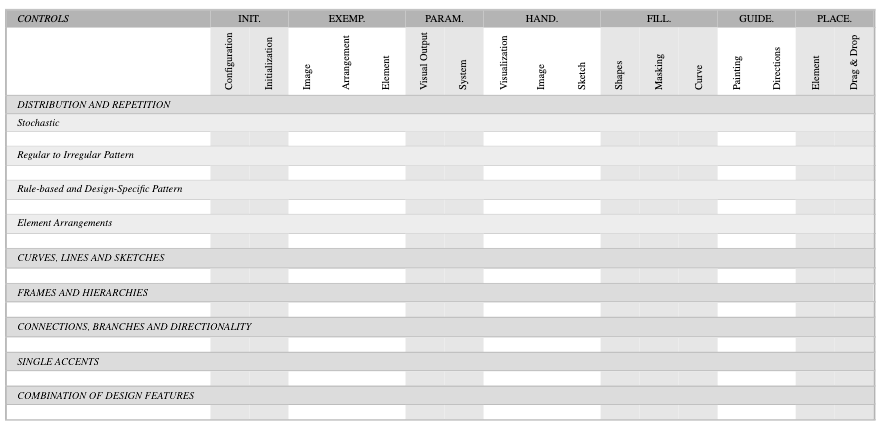
\includegraphics[width=\textwidth]{tables/table_all.png}
    \label{table:analysis}
    \caption[Control mechanisms in the state of the art]{Recent techniques are sorted by design areas and visual features they enable. For each work it is analysed and indicated which specific control mechanisms they offer.}
\end{figure*}




\subsection{Discussion of the Creative Means}
\label{subsec:analysis_creative_means}

\minortodo[inline]{Add intro}

\subsubsection{Example-Based Control}
\label{subsubsec:analysis_creative_means_example}

The investigation of example-based techniques shows valuable achievements for goal-oriented control and for increasing design spaces within specific contexts. With regard to creative control, in addition to the gain in \textit{variability} being a crucial step, the presented work also improves \textit{navigability} through interactive performances.

Element arrangements potentially enable greater visual variation because they do not need to adhere to any rule formulation. At the same time, the generation of a sample arrangement, usually done in an external application, is potentially tedious. A sample that is too small might lead to uniform results. Moreover, elements are often carefully connected in creative pattern designs, and might include a hierarchy of structures, such as for ornaments. Hence, element arrangements can only provide a subset - albeit an important one - of the design space needed for creative pattern generation.

The related work is overall uniform in working toward the classical requirements of finding the most efficient goal-oriented control 
%  as \Cref{table:analysis_example_creative} shows
. With the exception of \citeauthor*{ijiri_2008_aeb}~\cite{ijiri_2008_aeb} and \citeauthor*{galerne_2012_gne}~\cite{galerne_2012_gne} little effort has been made towards improving visual control for an artist. \citeauthor*{ma_2013_det}~\cite{ma_2013_det} present various powerful control functionalities but do not show their capabilities within an artist usable scenario. \citeauthor*{gilet_2012_map}~\cite{gilet_2012_map} also offer comparatively more mechanisms but as required configuration for their computation not necessarily as variable controllability.

Even if they are example-based, many techniques still require considerable non-creative effort for an artist, such as working with a power spectrum or predicting how changes in the exemplar, such as element arrangements, affect the output. The potential of these methods for creative control lies in furthering interactive performance, reducing initialization requirements and experimenting with the spatial influence of controls. The presented work only focuses on global designs, such as the whole canvas and repeating regions. Methods for which regions could be defined, models layered or the placement of single elements integrated constitute valuable directions for creative control mechanisms.


\subsubsection{Shapes and Masks}
\label{subsubsec:analysis_creative_means_shapes}

Procedural generation techniques offer novel systems that decouple control mechanisms from the implementation of individual models. This enables more possible results for one specific technique, thus improving the size of design spaces. 
% , as~\Cref{table:analysis_shape} shows. 
Sophisticated masks and growth constraints lead to visually interesting and complex designs. However, it is not directly predictable how a space will be filled exactly. Because most of the presented methods only offer quite limited interactive performance, even  a basic trail and error exploration is hardly feasible; hence, the navigation of the design space becomes cumbersome, and stimulation becomes hindered. The one technique \cite{santoni_2016_ggp} that offers the means for a transparent navigation is also the one with the most restricted design space. \citeauthor*{santoni_2016_ggp}~\cite{santoni_2016_ggp}s' consideration of a navigation history stands out from all related work in this survey. In terms of stimuli, the mass-spring system for editing control guides offered by \citeauthor*{benes_2011_gpm}~\cite{benes_2011_gpm} is a promising direction because it is intuitive, enjoyable to use and encourages exploration.

In terms of control mechanisms for a more complex design goal, these techniques do not permit hierarchical or element-level local controls or the control of element connections needed by artists who want to generate patterns creatively without having to write code.


\subsubsection{Vector Fields}
\label{subsubsec:analysis_creative_means_fields}

The discussed work 
% in \Cref{table:analysis_vectorfield} 
shows that fields allow for greater visual variation by opening the design space and transparent control for filling a space automatically. When designing a vector field, artists do not work with the pattern directly, but fields are intuitive to understand. Their abstraction translates to the model in a straightforward manner. Thus, using flow within a vector field to design is a suitable control mechanism, especially for designs that aims to align their elements to the space.

\subsubsection{Curves, Sketches and Painting}
\label{subsubsec:analysis_creative_means_curves}

Curves and sketch-like methods offer a well communicated, hence transparent navigation. 
% , as~\Cref{table:analysis_shape} shows. 
The discussed techniques are mostly interactive, artists are familiar with their functionality from the real world and they work directly on the canvas. The ease and directness of usage also constitute a foundation for possible immersive flow of work. Using painting-like methods can allow for smoother navigation by integrating brush settings and increasing the quantity of controls.

However, because creation techniques and design spaces are open, it could lead to manual and tedious creation requirements for patterns, such as when filling a background. Here, the incorporation of procedural creation principles for automatic fillings into a data-driven process by \citeauthor*{kazi_2012_vit}~\cite{kazi_2012_vit} and \citeauthor*{xing_2014_apr}~\cite{xing_2014_apr} is a promising direction. Instead of fostering a free painting-like quality, design principles for pattern designs could be added to create a more organized output.

\subsubsection{Element Placement}
\label{subsubsec:analysis_creative_means_elements}

Element placement control mechanisms are closely related to the data-driven sketch-based techniques, and it shows a further promising approach for integrating procedural modeling functionalities into a data-driven process. 
% As \Cref{table:analysis_elementplacement} shows,
\citeauthor*{guerrero_2016_pep}~\cite{guerrero_2016_pep} present a overall transparently navigable and stimulating control mechanism. With a carefully designed workflow, it further fosters an artist stimulation by offering novel but suitable design variations.

